\section{Descoberta de Conhecimento}
A primeira vez que apareceu o termo \textit{Descoberta de Conhecimento em Banco de Dados} (do inglês \textit{Knowledge Discovery in Database}) foi em 1989, por Piatetsky-Shapiro, com o objetivo de enfatizar que o produto final do processo é o conhecimento.

Para \cite{fayyad:1996} KDD refere-se ao processo geral de descobrir conhecimento útil a partir dos dados, essa extração de conhecimento é um processo não-trivial. 
A Figura ~\ref{fig:kdd} mostra o processo de KDD proposto por Fayyad et al. 
O termo processo implica que o KDD é composto por várias etapas, as quase são iterativas e interativas. 
Iterativa reflete o ciclo entre as etapas e, interativa reflete o caráter interdisciplinar do processo, uma vez que o KDD se aplica em inúmeras áreas e para resolver o problema muitas vezes é necessária a ajuda de um \textit{expert} naquela área.

A seguir, será dada uma visão geral de cada uma das fases.


\begin{figure}
    \centering
    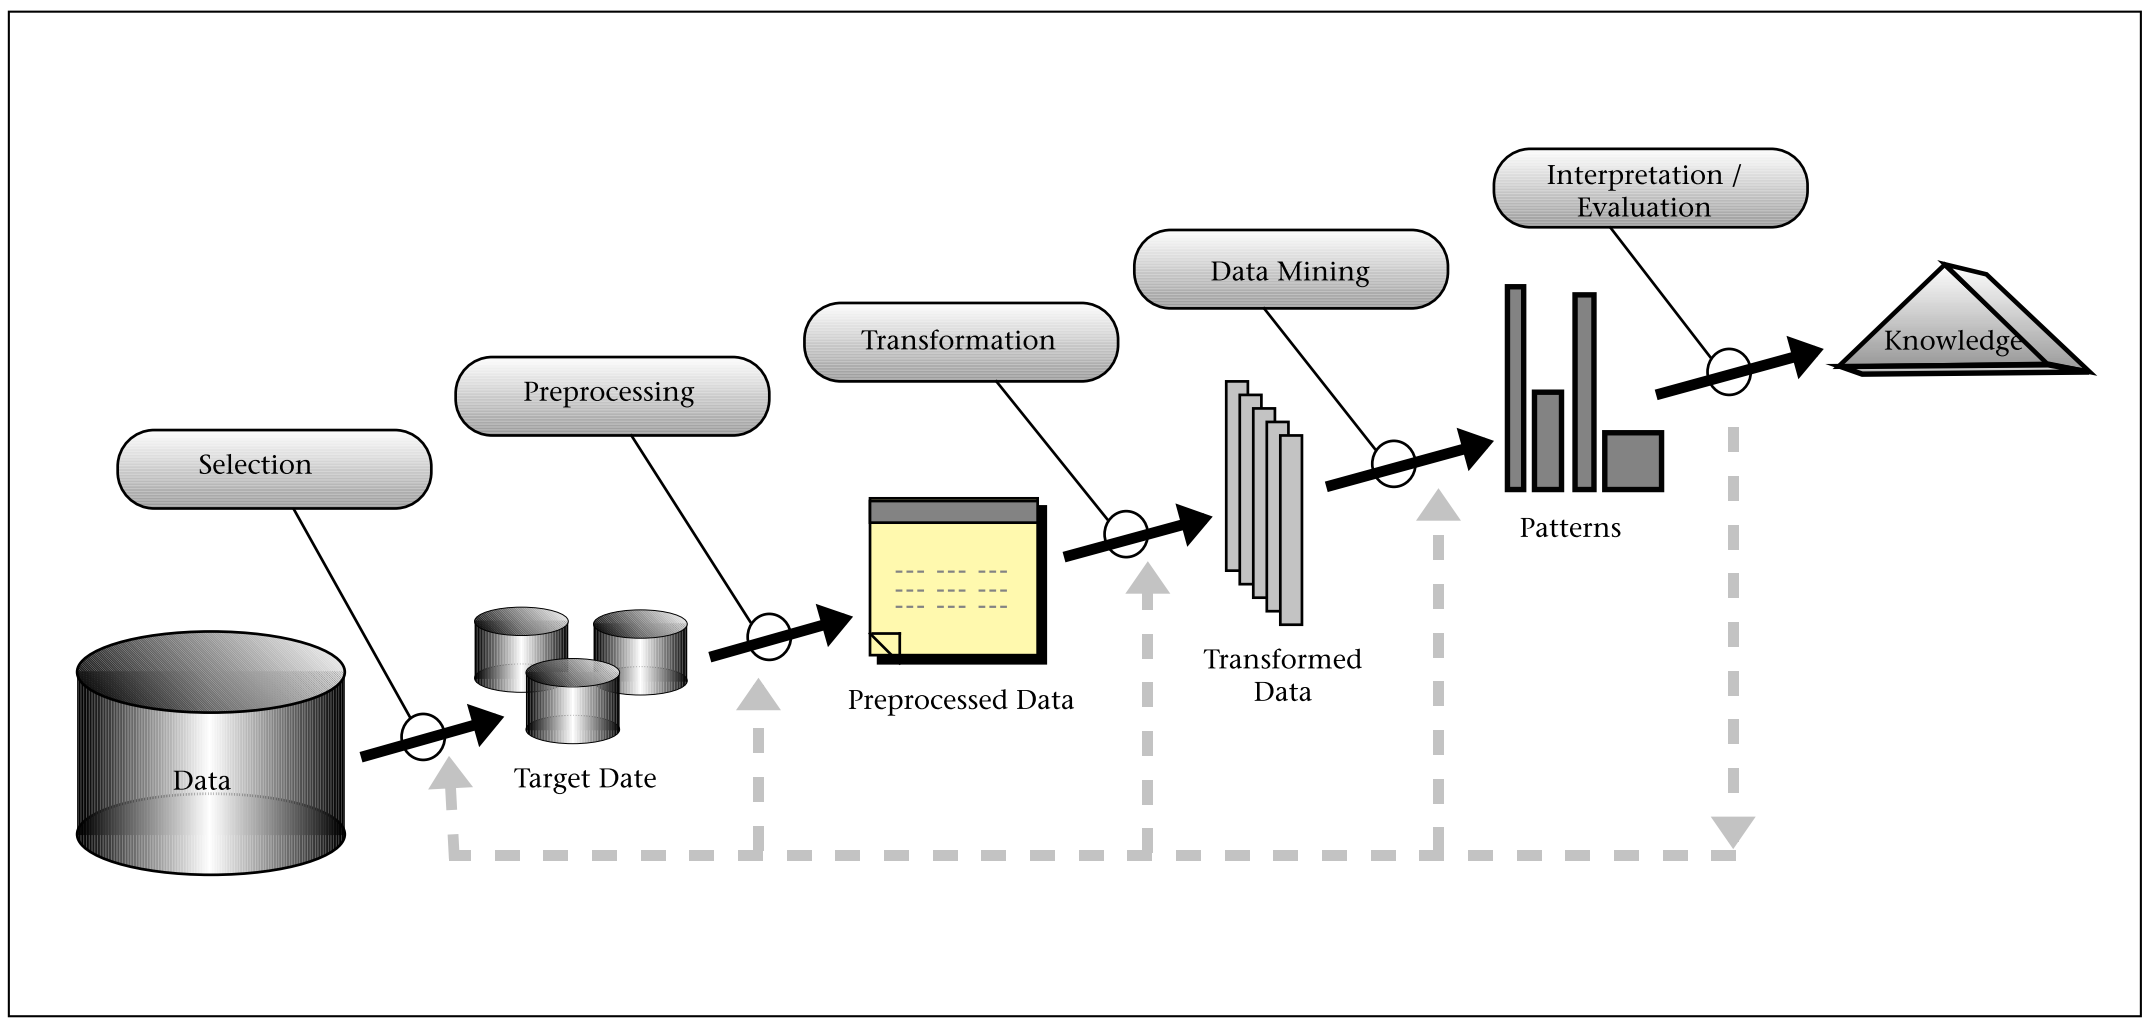
\includegraphics[scale=0.39]{Imagens/kdd.png}
    \caption{Processo de KDD (Fayyad et al)}
    \label{fig:kdd}
\end{figure}

\subsection{Fases do KDD}
% --- SELEÇÃO --- %
\textbf{1) Seleção}: A primeira etapa no processo é chamada de seleção, que é responsável por selecionar um \textit{dataset} a partir de uma base de dados maior. A escolha desse \textit{dataset} dependerá do domínio do problema que está tentando resolver. Em geral, a escolha é feita por um especialista ou por algum algoritmo de extração de características. O conjunto de dados selecionado é chamado de \textit{Target Data}.

% --- PRÉ-PROCESSAMENTO -- %
\textbf{2) Pré-processamento}: Após ter o conjunto de dados a ser utilizado, é comum que esses dados não estejam em boa qualidade, dessa forma, é necessário tratá-los e limpá-los. Operações básicas realizadas nesse nível devem lidar com:

\begin{itemize}[leftmargin=1.2cm]
    \begin{description}[font=$ \bullet $]
        \item [ Valores faltantes] Valores nulos. Ocorre quando alguém deixa um campo de um formulário em branco, por exemplo.
        \item [ \textit{Outliers}] Quando um valor foge muito do padrão dos dados. Deve ser identificado e eliminado do conjunto de dados.
        \item[ Dados derivados] Ocorre quando um dado pode ser obtido a partir de outro. Por exemplo, a idade de um indivíduo pode ser obtida a partir do seu ano de nascimento, dessa forma, não faz muito sentido ter esses dois atributos no conjunto de dados.
    \end{description}
\end{itemize}

% --- TRANSFORMAÇÃO -- %
\textbf{3) Transformação}: Uma vez que os dados estão limpos e tratados, é necessário armazená-los e formatá-los adequadamente para que os algoritmos de aprendizado possam ser utilizados. A título de exemplo, se for usar um algoritmo de agrupamento baseado na distância euclidiana, é necessário converter todos os dados para numérico.

% --- MINERAÇÃO DE DADOS -- %
\textbf{4) Mineração de Dados}:  Embora todas as etapas sejam importantes, a etapa de Mineração de Dados é a que recebe maior atenção. Conforme \cite{fayyad:1996}, mineração de dados é a aplicação de algoritmos específicos para extrair padrões a partir dos dados. Ainda de acordo com Fayyad et al, os algoritmos de mineração de dados podem ser dividimos em cinco categorias: Associação, Classificação, Regressão, Segmentação e Sumarização. A tarefa na qual este projeto se encontra é a de classificação. 

A tarefa de classificação é responsável por identificar a qual classe um determinado registro pertence. Inicialmente, o modelo é "alimentado" com conjunto de registros já rotulados, isto é, é fornecida a qual classe os registros pertencem. Com esses dados, o algoritmo treina a aprende padrões que fazem com que um registro pertença a uma classe ou a outra
(esse tipo de aprendizado é conhecido como aprendizado supervisionado).


% -- INTERPRETAÇÃO/VALIDAÇÃO -- %
\textbf{5) Interpretação/Validação}: Uma vez que o modelo já foi treinado, é medido a sua capacidade de generalização. Nesta etapa é fundamental a presença do especialista, visto que, a melhor métrica de avaliação dependerá do negócio. Caso o desempenho não seja satisfatório, é possível retornar para qualquer etapa no processo de KDD, e o ciclo recomeça até chegar a um modelo que satisfaça o negócio.





